%%%%%%%%%%%%%%%%%%%%%%%%%%%%%%%%%%%%%%%%%%%%%%%%%%%%%%%%%%%%%%%%%%%%
% Poster template for Master Projects
% Creation: September 17, 2008
% Modified: October 10, 2008
% Authors: Erik Steur and Rob Mestrom (WH -1.144)
%%%%%%%%%%%%%%%%%%%%%%%%%%%%%%%%%%%%%%%%%%%%%%%%%%%%%%%%%%%%%%%%%%%%

\documentclass[a4paper,12pt]{article}
\usepackage[a4,wtbuk,themedarkblue]{tuepdfscreen2008}
\usepackage[english]{babel}
\usepackage{amsmath,amssymb}
%\usepackage{mathtime}     % This package is not required, it loads Mathtime fonts for mathematical formulas which I prefer.
%\usepackage{framed}         % Used for textboxes
%\usepackage{wrapfig}        % Used to wrap figures
\usepackage{graphicx}
\usepackage{enumitem}
\usepackage[font=footnotesize,labelfont=bf]{caption}

%% For posterboxes?
%\usepackage[orientation=portrait,size=a4,scale=1.0]{beamerposter}

\usepackage[tikz]{bclogo}
\renewcommand \logowidth{0pt}
\newcommand{\emptylogo}{
\includegraphics[width=0pt]{Figures/Empty}}

%% To turn Figure into Fig.
%\renewcommand{\figurename}{Fig.}
%\addto\captionsenglish{\renewcommand{\figurename}{Fig.}}

%\usepackage[framemethod=tikz]{mdframed}
%\usepackage[style=1]{mdframed}
%\newcommand\Loadedframemethod{TikZ}
%\usepackage[framemethod=\Loadedframemethod]{mdframed}
%\newmdtheoremenv [
%    outerlinewidth = 2 ,
%    leftmargin = 40 ,
%    rightmargin = 40 ,
%    backgroundcolor = yellow ,
%    outerlinecolor = blue ,
%    innertopmargin = \topskip ,
%    splittopskip = \topskip ,
%    ntheorem = true ,
%    skipabove = \baselineskip ,
%    skipbelow = \baselineskip ]
%    {theorem}{Theorem}[section]

%% Tikz
%\usepackage{tikz}
%\usetikzlibrary{backgrounds}


%%%%%%%%%%%%%%%%%%%%%%%%%%%%%%%%%%%%%%%%%%%%%%%%%%%%%%%%%%%%%%%%%%%%
% Correct hyphenation
%%%%%%%%%%%%%%%%%%%%%%%%%%%%%%%%%%%%%%%%%%%%%%%%%%%%%%%%%%%%%%%%%%%%
\hyphenation{off-line}

%%%%%%%%%%%%%%%%%%%%%%%%%%%%%%%%%%%%%%%%%%%%%%%%%%%%%%%%%%%%%%%%%%%%
% Modify itemize
%%%%%%%%%%%%%%%%%%%%%%%%%%%%%%%%%%%%%%%%%%%%%%%%%%%%%%%%%%%%%%%%%%%%
%[itemsep = 0pt, parsep = 0pt]
%\newenvironment{my_itemize}{
%\begin{itemize}
%  \setlength{\topsep}{0pt}
%  \setlength{\leftmargin}{-0.5cm}%{0pt}
%  \setlength{\itemindent}{0pt}%{-0.5cm}%{0pt}
%  \setlength{\parindent}{-0.5cm}%{0pt}
%  \setlength{\itemsep}{0pt}
%  \setlength{\parskip}{0pt}
%  \setlength{\parsep}{0pt}}
%{\end{itemize}
%}
%\setlist[itemize]{noitemsep, topsep=0pt, leftmargin=-0.5cm, itemindent=-0.5cm, parindent=-0.5cm, itemsep=0pt, parskip=0pt, parsep=0pt}

%%%%%%%%%%%%%%%%%%%%%%%%%%%%%%%%%%%%%%%%%%%%%%%%%%%%%%%%%%%%%%%%%%%%
% Logos and title layout
%%%%%%%%%%%%%%%%%%%%%%%%%%%%%%%%%%%%%%%%%%%%%%%%%%%%%%%%%%%%%%%%%%%%

% Insert company logo (max height approximately 14 mm)
%% PDF
\setstatustext{
\includegraphics[height=14mm]{Figures/logoAtHome}\hspace{1.5cm}
\includegraphics[height=14mm]{Figures/logo_european_open}}

%% DVI
%\setstatustext{
\includegraphics[height=14mm, bb = 0 0 458 266]{Figures/logoAtHome.png}\hspace{3.0cm}\includegraphics[height=14mm,bb = 0 0 670 175]{Figures/RoboCup2013logo.png}}
% If no company logo is needed, uncomment the following line
%\setstatustext{}

%\Committee{
\includegraphics[height=35mm]{Figures/techunitedlogo} }
\Committee{
\includegraphics[height=45mm]{Figures/techunitedlogo} }

\begin{document}
\begin{slidetop}

%%%%%%%%%%%%%%%%%%%%%%%%%%%%%%%%%%%%%%%%%%%%%%%%%%%%%%%%%%%%%%%%%%%%
% [Author] and {Title} of the poster
%%%%%%%%%%%%%%%%%%%%%%%%%%%%%%%%%%%%%%%%%%%%%%%%%%%%%%%%%%%%%%%%%%%%
%\slidetitle[RoboCup~2015, Hefei, China]{\vspace{10mm} Tech United Eindhoven}
\slidetitle[RoboCup~European~Open, Eindhoven, Netherlands]{\vspace{10mm} Tech United Eindhoven}

\begin{multicols}{2}

%\section*{\large AMIGO}
%\begin{bclogo}[couleur = white, arrondi = 0.25, couleurBord = tuedarkblue, epBarre = 0]{\textcolor{tuedarkblue}{AMIGO}}
\begin{bclogo}[couleur = white, arrondi = 0.25, couleurBord = tuedarkblue, epBarre = 0, logo=\emptylogo]{\textcolor{tuedarkblue}{AMIGO \& SERGIO}}
\bigskip
\begin{minipage}[T]{0.48\linewidth}
%	\vspace{-0.4cm}
	\begin{center}
		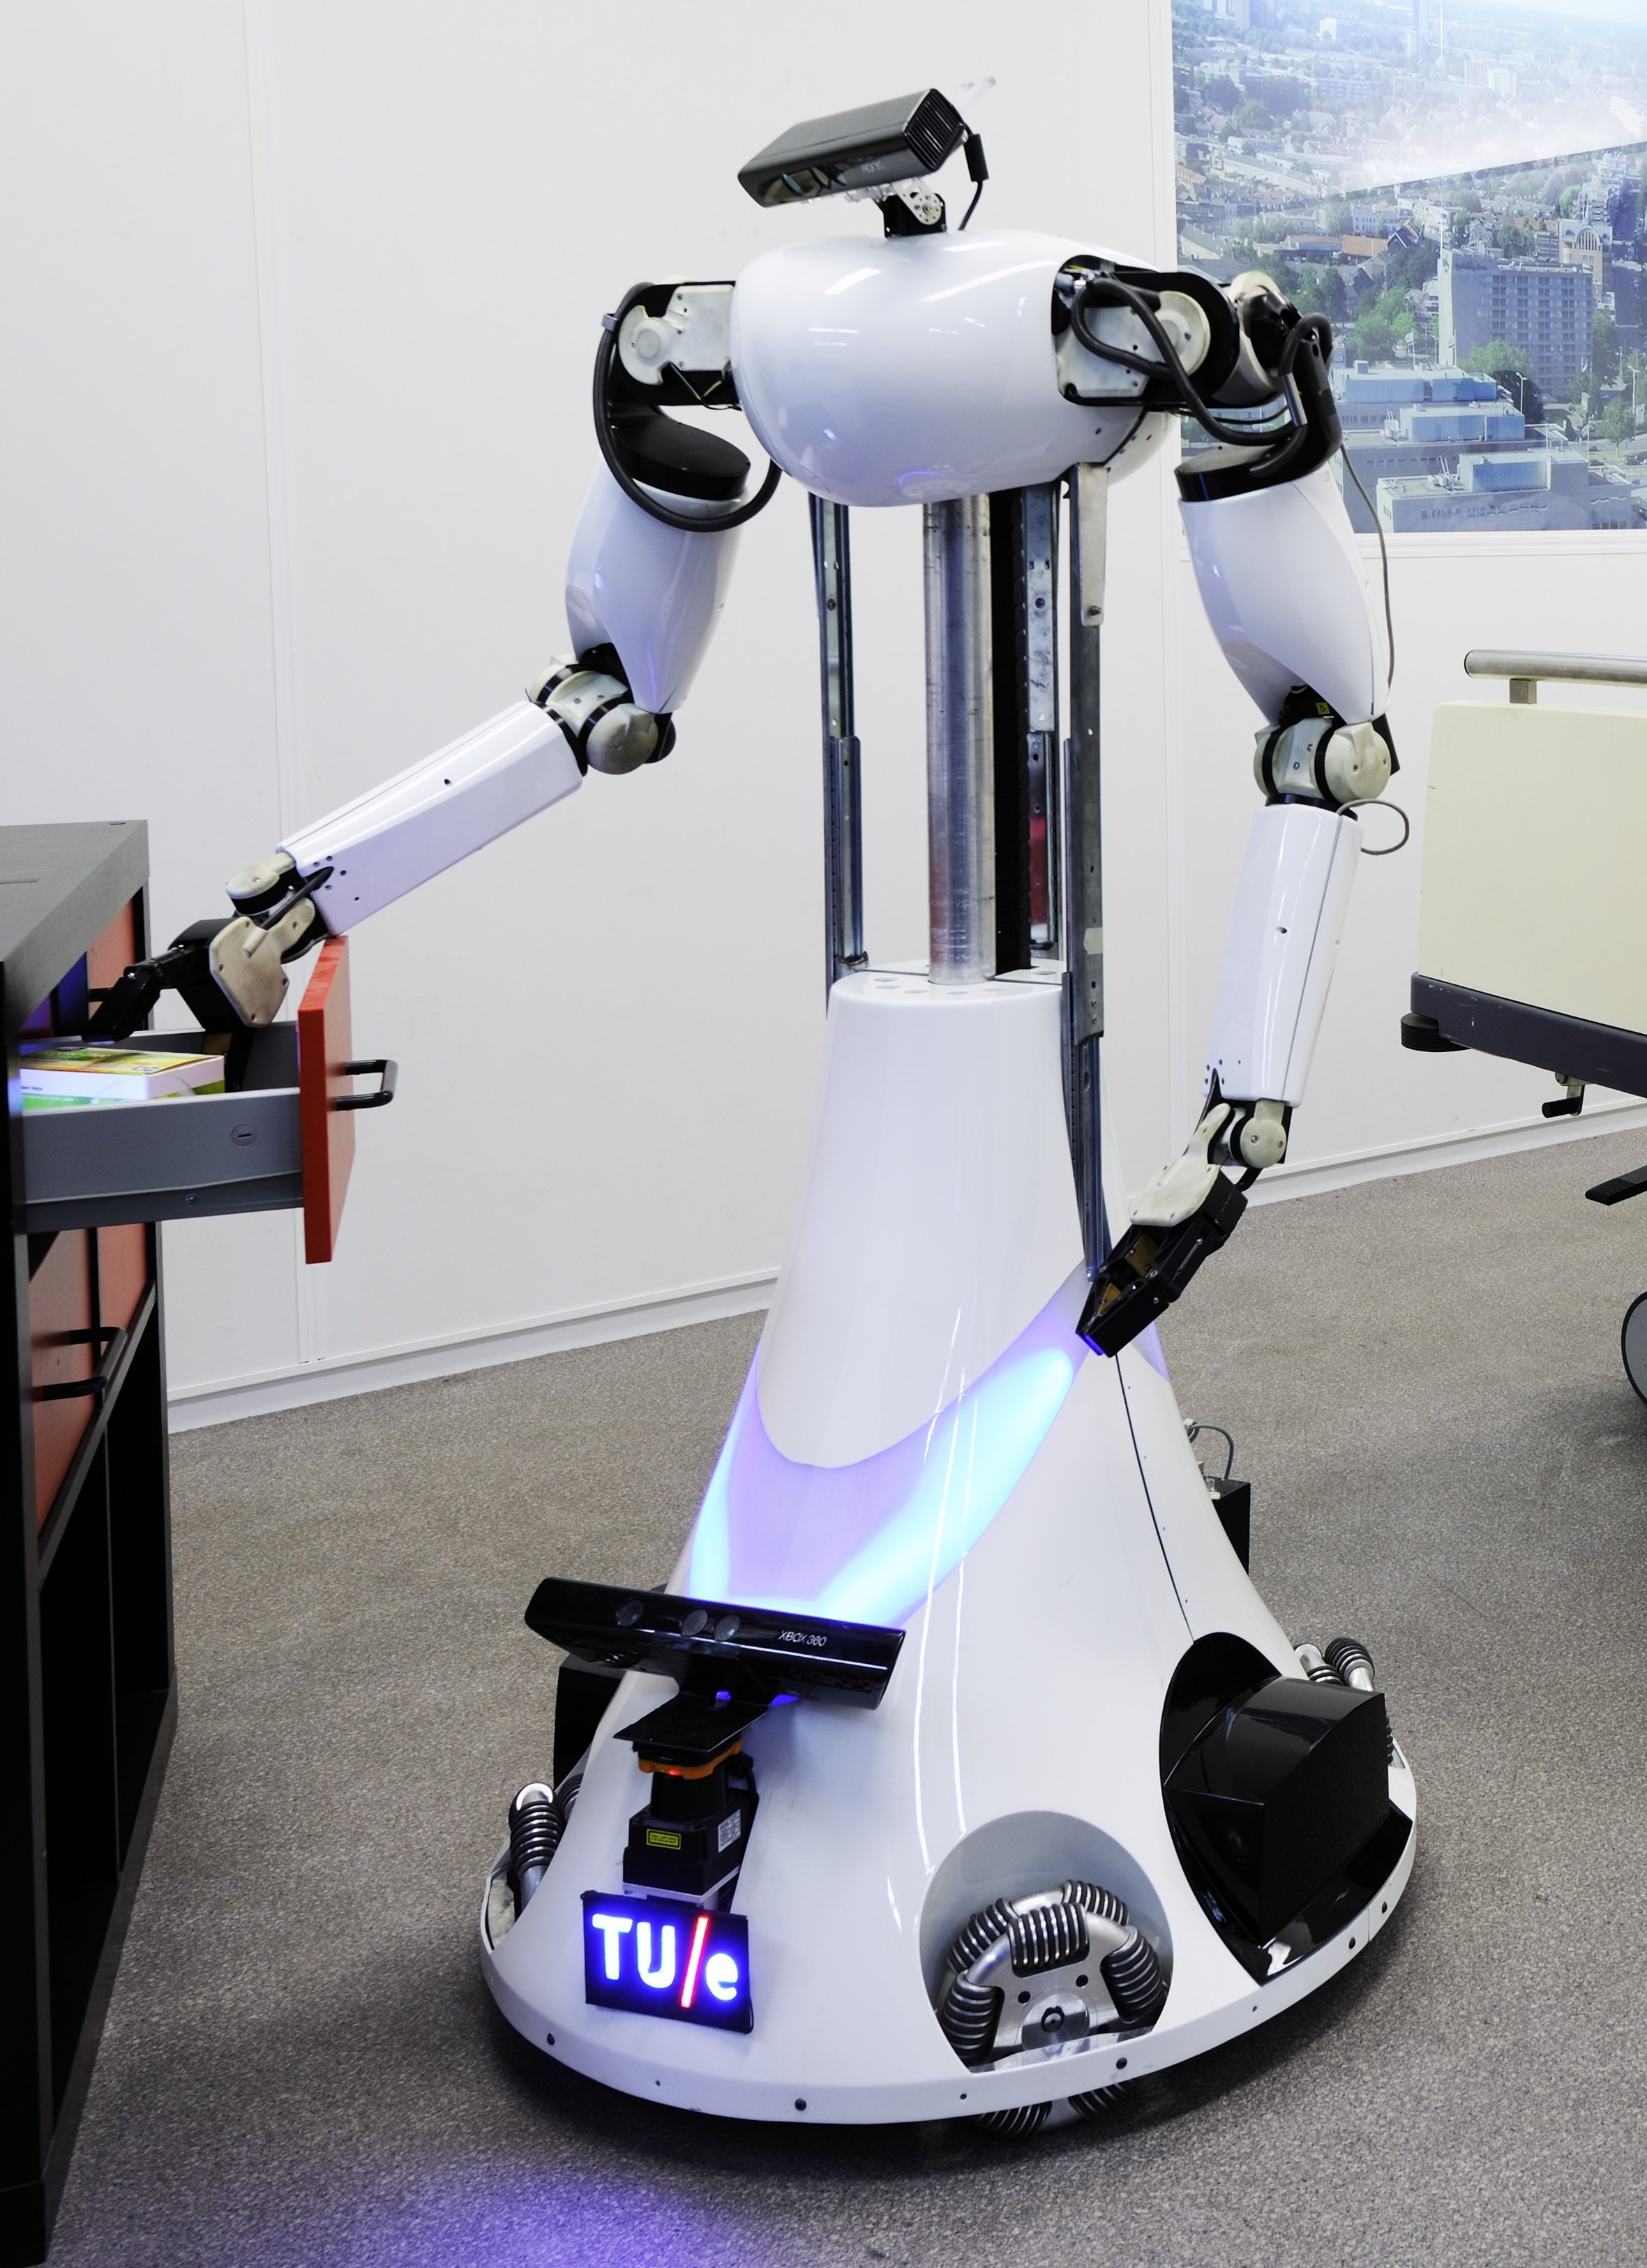
\includegraphics[height=4cm]{Figures/amigo_hospital72}
		\figcaption{AMIGO}
	\end{center}
\end{minipage}
\hfill
\begin{minipage}[T]{0.48\linewidth}
%    \vspace{-0.4cm}
    \begin{center}
    	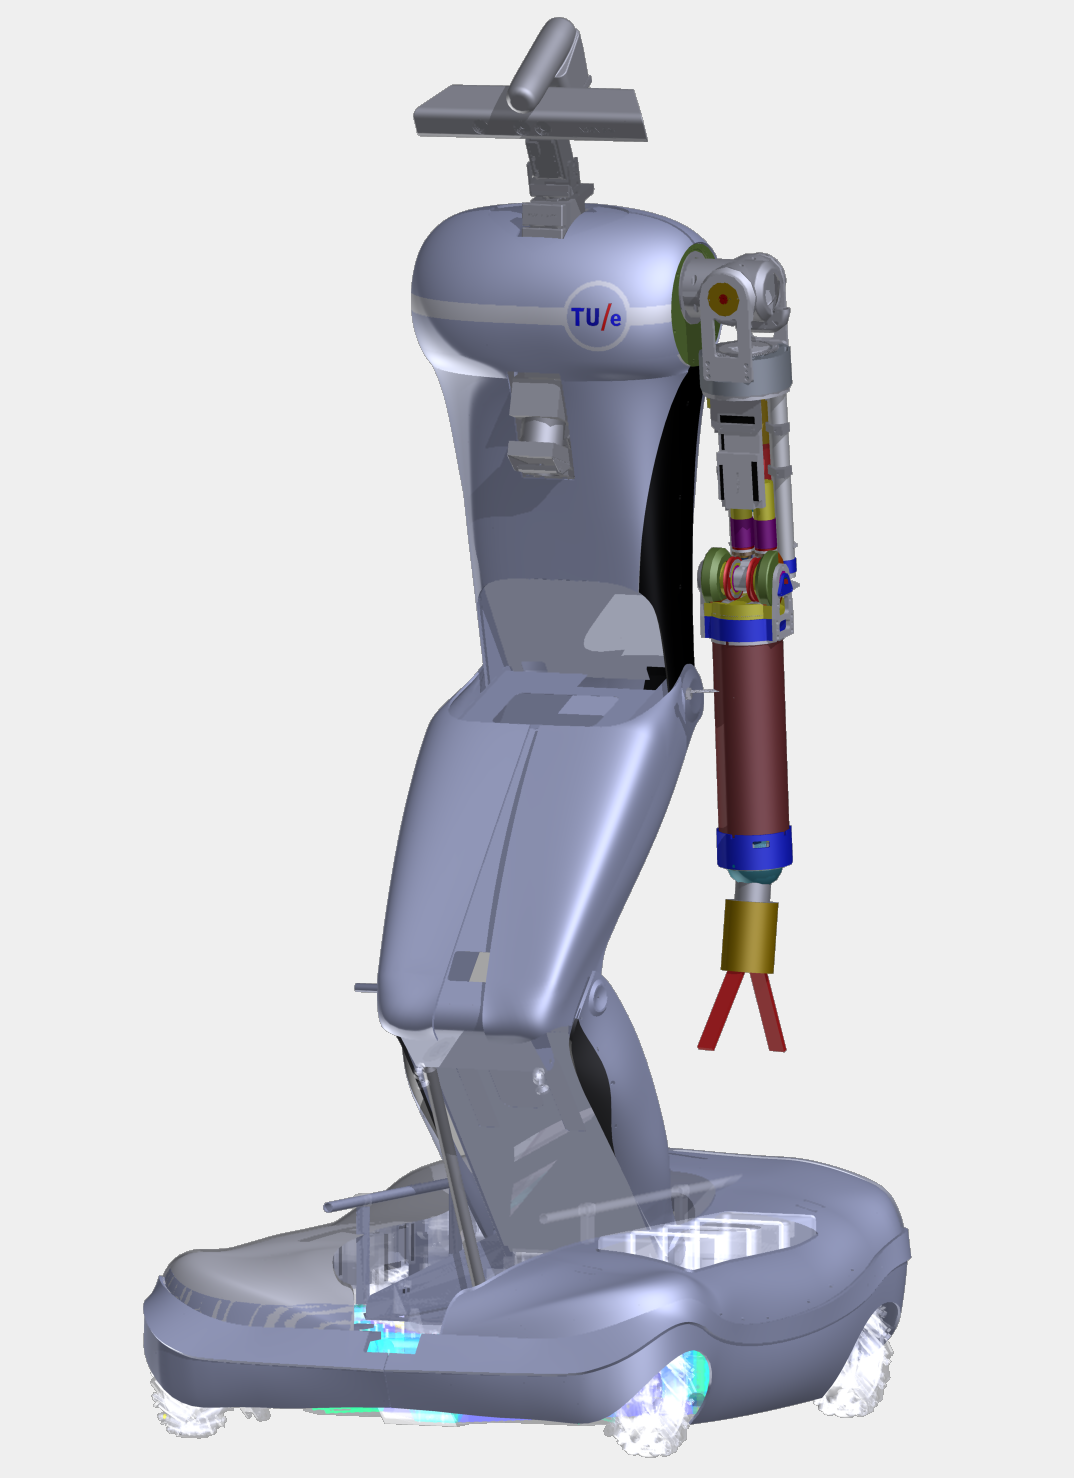
\includegraphics[height=4cm]{Figures/SERGIO}
        \figcaption{SERGIO}
    \end{center}
\end{minipage}
    \begin{itemize}[itemsep = 0pt, parsep = 0pt, leftmargin=15pt]
    	\item AMIGO
    	\begin{itemize}[itemsep = 0pt, parsep = 0pt, leftmargin=15pt]
    		\item Omni-wheels, 1 DoF torso
    	\end{itemize}
    	\item SERGIO
    	\begin{itemize}[itemsep = 0pt, parsep = 0pt, leftmargin=15pt]
    		\item Suspended mecanum wheels, 2 DoF torso
    	\end{itemize}
        \item 7-DoF manipulators
        \item Designs available at Robotic Open Platform
    \end{itemize}
\end{bclogo}
\vspace{0.2cm}
\begin{bclogo}[couleur = white, arrondi = 0.25, couleurBord = tuedarkblue, epBarre = 0, logo=\emptylogo]{\textcolor{tuedarkblue}{World modeling}}
\bigskip
\begin{center}
	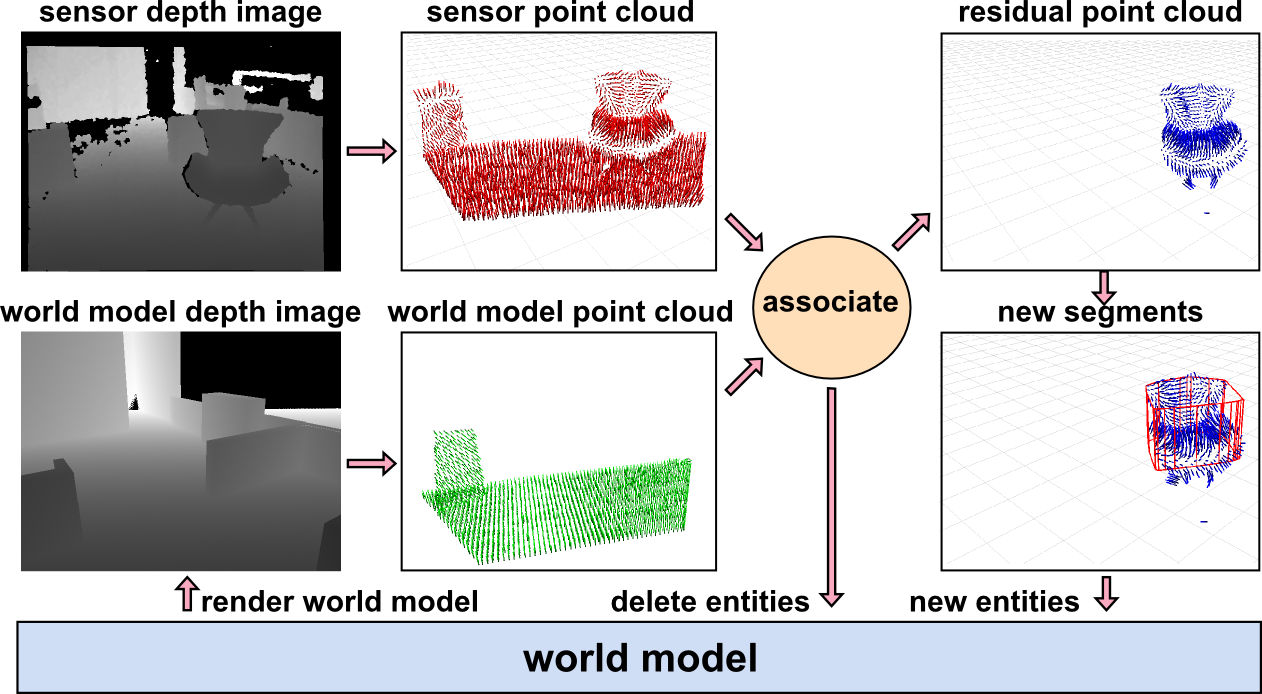
\includegraphics[width=0.9\linewidth]{Figures/ed_pipeline}
	\figcaption{Overview of ED: Environment Descriptor}
\end{center}
\begin{itemize}[itemsep = 0pt, parsep = 0pt, leftmargin=15pt]
%	\item One single object-oriented, volumetric world model, used for:
	\item A central object-oriented, volumetric world model, used for:	
	\begin{itemize}[itemsep = 0pt, parsep = 0pt, leftmargin=15pt]
		\item Navigation
		\item Object tracking
		\item Localization
	\end{itemize}
	\item Objects have 3D shape, pose, type
	\item Updating by comparing rendered world model with depth image
\end{itemize}
\end{bclogo}

\begin{bclogo}[couleur = white, arrondi = 0.25, couleurBord = tuedarkblue, epBarre = 0, logo=\emptylogo]{\textcolor{tuedarkblue}{Furniture fitting}}
\bigskip
\begin{center}
	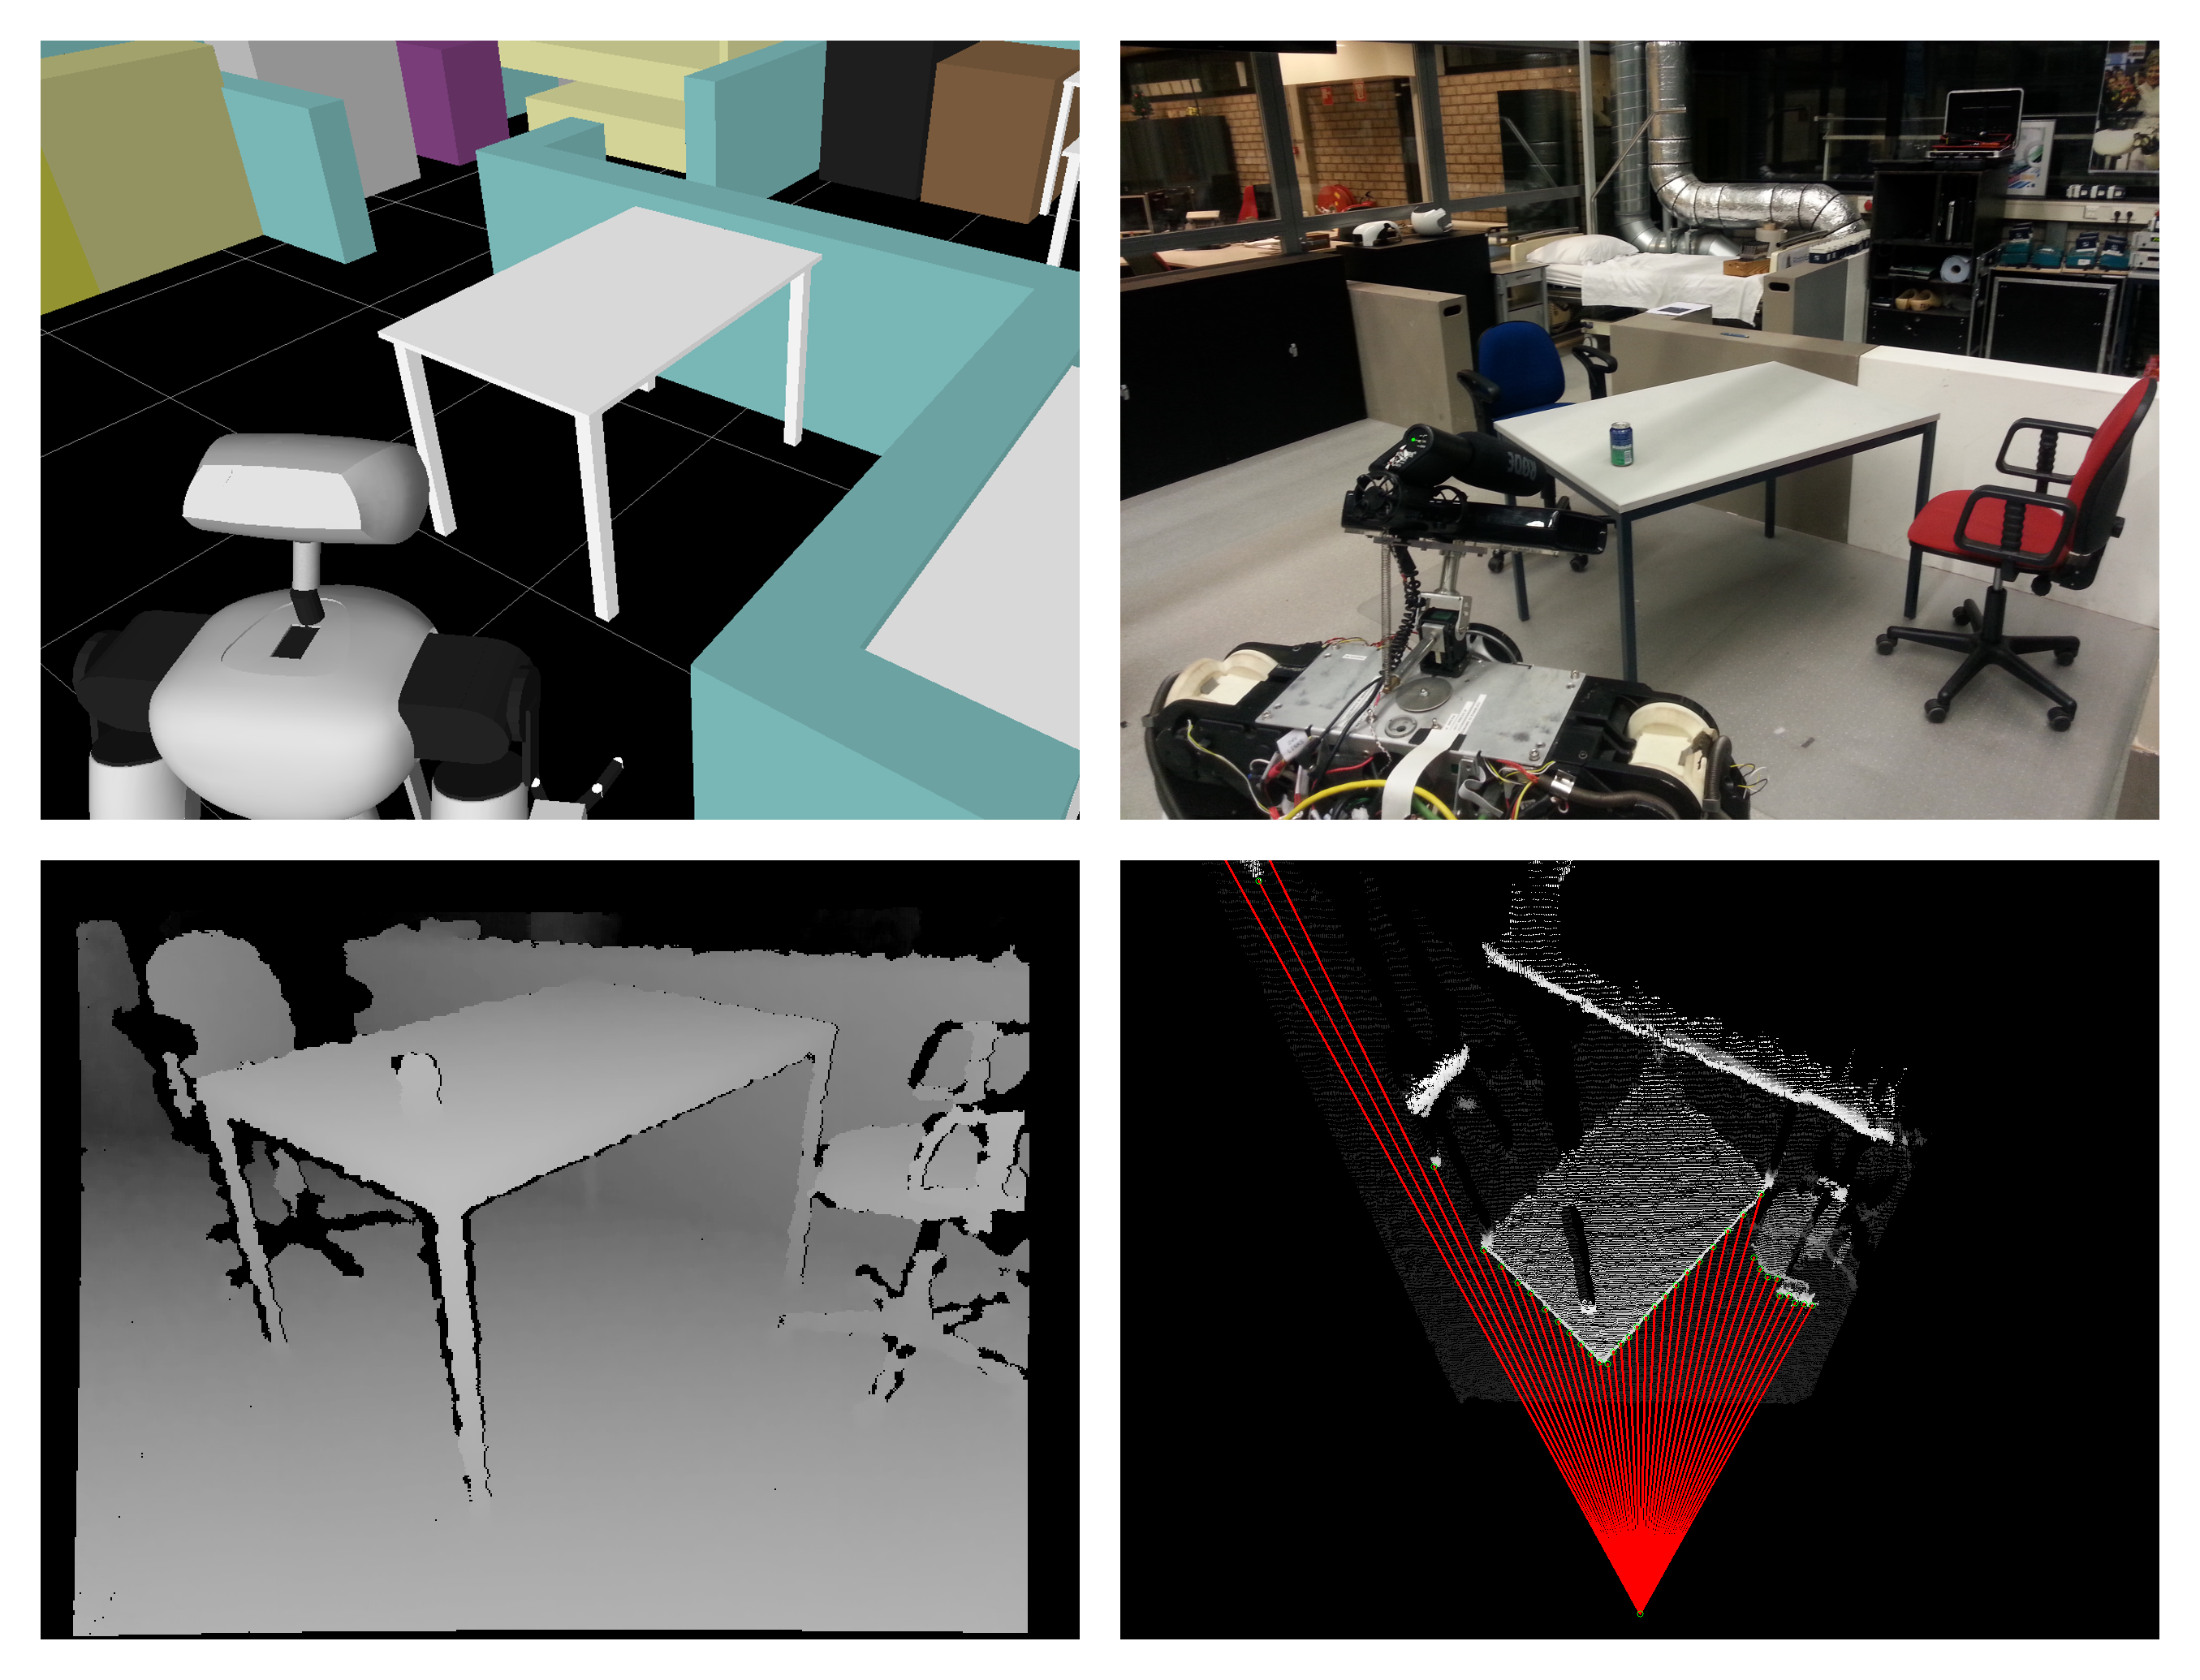
\includegraphics[width=0.9\linewidth]{Figures/fitting}
%	\figcaption{
%		Overview of the WebGUI architecture.
%		The robot's functionalities are exposed with the Robot API that is implemented in JavaScript.
%		The webserver that is hosting the GUI connects this Robot API to a graphical user interface that is offered to multiple clients on different platforms.}
%	\label{fig:webgui_architecture}
\end{center}
%\begin{minipage}[T]{0.3\textwidth}
%	\begin{center}
%		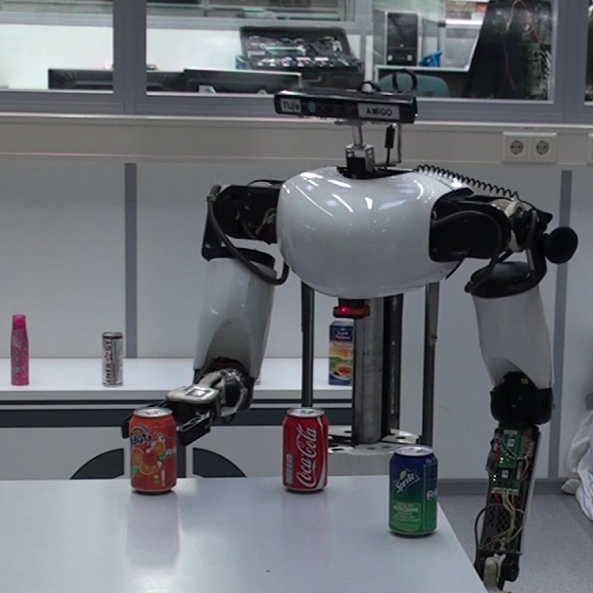
\includegraphics[width=1\linewidth]{Figures/pickup_object}
%		\figcaption{Pick up task}
%	\end{center}
%\end{minipage}
%\hfill
%\begin{minipage}[T]{0.3\textwidth}
%	\begin{center}
%		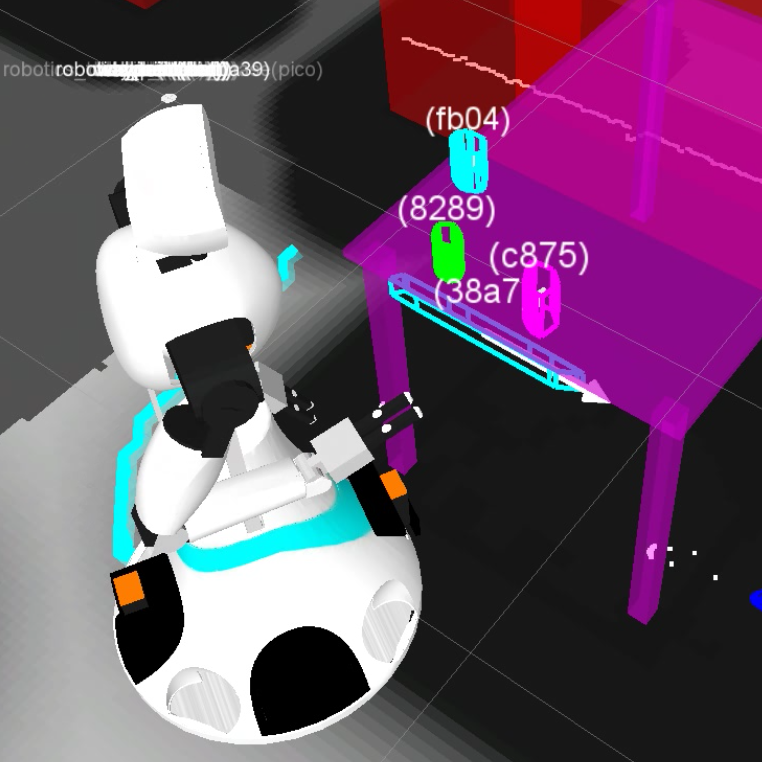
\includegraphics[width=1\linewidth]{Figures/pickup_object_world_model}
%		\figcaption{World model}
%	\end{center}
%\end{minipage}
%\hfill
%\begin{minipage}[T]{0.3\textwidth}
%	\begin{center}
%		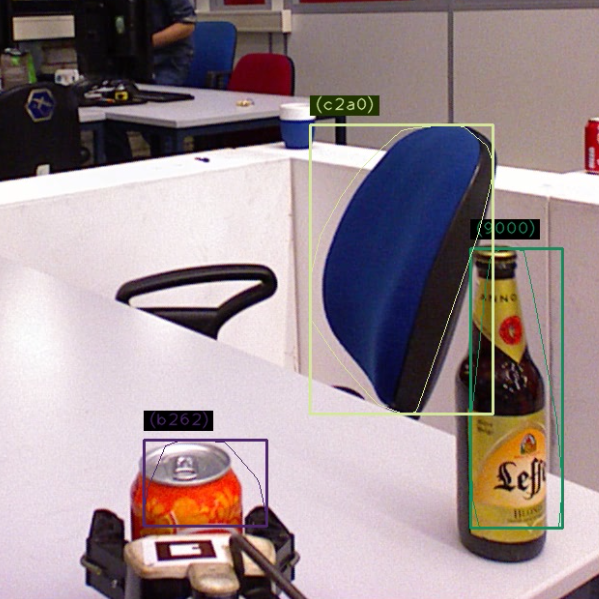
\includegraphics[width=1\linewidth]{Figures/pick_up_kinect_view}
%		\figcaption{Sensor view}
%	\end{center}
%\end{minipage}
\begin{itemize}[itemsep = 0pt, parsep = 0pt, leftmargin=15pt]
	\item Updating the pose of furniture objects in the world model
	\begin{itemize}[itemsep = 0pt, parsep = 0pt, leftmargin=15pt]
		\item Navigation map and locations are updated
		\item Object segmentation is robustified
	\end{itemize}
	\item Efficient fitting by projecting the 3D point cloud to a 1D range array
%	\item Combination of weak classifiers:
%	\begin{itemize}[itemsep = 0pt, parsep = 0pt, leftmargin=15pt]
%		\item Size
%		\item SIFT
%		\item Color histogram
%		\item Contour
%		\item Face detection
%	\end{itemize}
%	\item Asynchronous recognition and labeling of entities 
%	\begin{itemize}[itemsep = 0pt, parsep = 0pt, leftmargin=15pt]
%		\item Each entity has one threaded perception worker
%	\end{itemize}
\end{itemize}
\end{bclogo}
\vspace{0.2cm}
%\section*{\large Motion Planning}
\begin{bclogo}[couleur = white, arrondi = 0.25, couleurBord = tuedarkblue, epBarre = 0, logo=\emptylogo]{\textcolor{tuedarkblue}{WebGUI}}
\bigskip
\begin{center}
	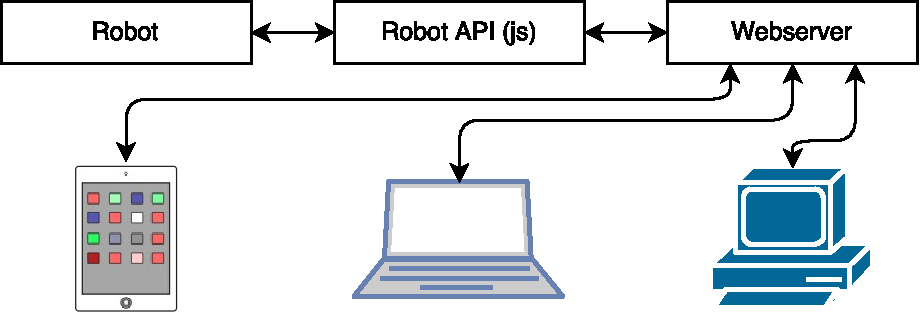
\includegraphics[width=0.9\linewidth]{Figures/webgui_architecture}
%	\figcaption{
%		Overview of the WebGUI architecture.
%		The robot's functionalities are exposed with the Robot API that is implemented in JavaScript.
%		The webserver that is hosting the GUI connects this Robot API to a graphical user interface that is offered to multiple clients on different platforms.}
%	\label{fig:webgui_architecture}
\end{center}
%\begin{center}
%	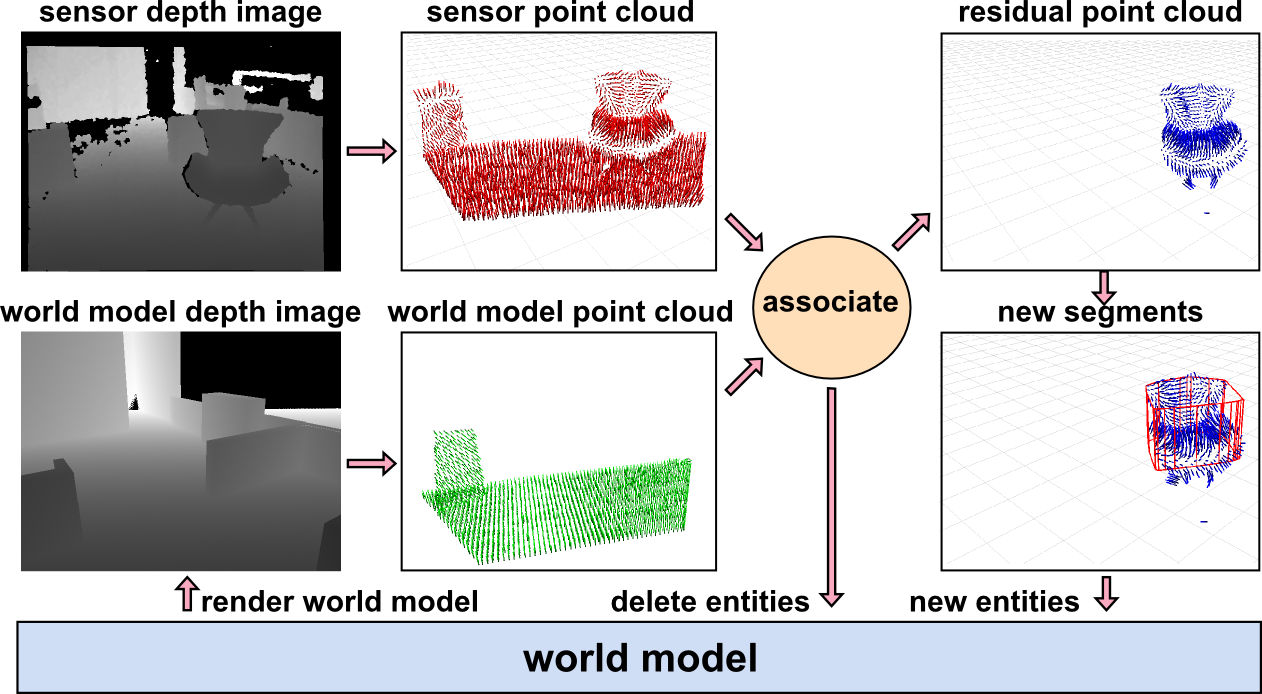
\includegraphics[width=0.9\linewidth]{Figures/ed_pipeline}
%	\figcaption{Overview of ED: Environment Descriptor}
%\end{center}
\begin{itemize}[itemsep = 0pt, parsep = 0pt, leftmargin=15pt]
%%	\item One single object-oriented, volumetric world model, used for:
%	\item A central object-oriented, volumetric world model, used for:	
%	\begin{itemize}[itemsep = 0pt, parsep = 0pt, leftmargin=15pt]
%		\item Navigation
%		\item Object tracking
%		\item Localization
%	\end{itemize}
%	\item Objects have 3D shape, pose, type
%	\item Updating by comparing rendered world model with depth image
	\item Web-based Graphical User Interface
	\item Cross-platform
	\item Action server schedules the robot's tasks based on user input
\end{itemize}
\end{bclogo}

%\section*{\large Reasoning and World Modeling}
%\vspace{1cm}
\vfill
%\section*{\large Perception}
\begin{bclogo}[couleur = white, arrondi = 0.25, couleurBord = tuedarkblue, epBarre = 0, logo=\emptylogo]{\textcolor{tuedarkblue}{Natural language interpretation}}
\bigskip
%\begin{minipage}[T]{0.48\textwidth}
%    \begin{center}
%        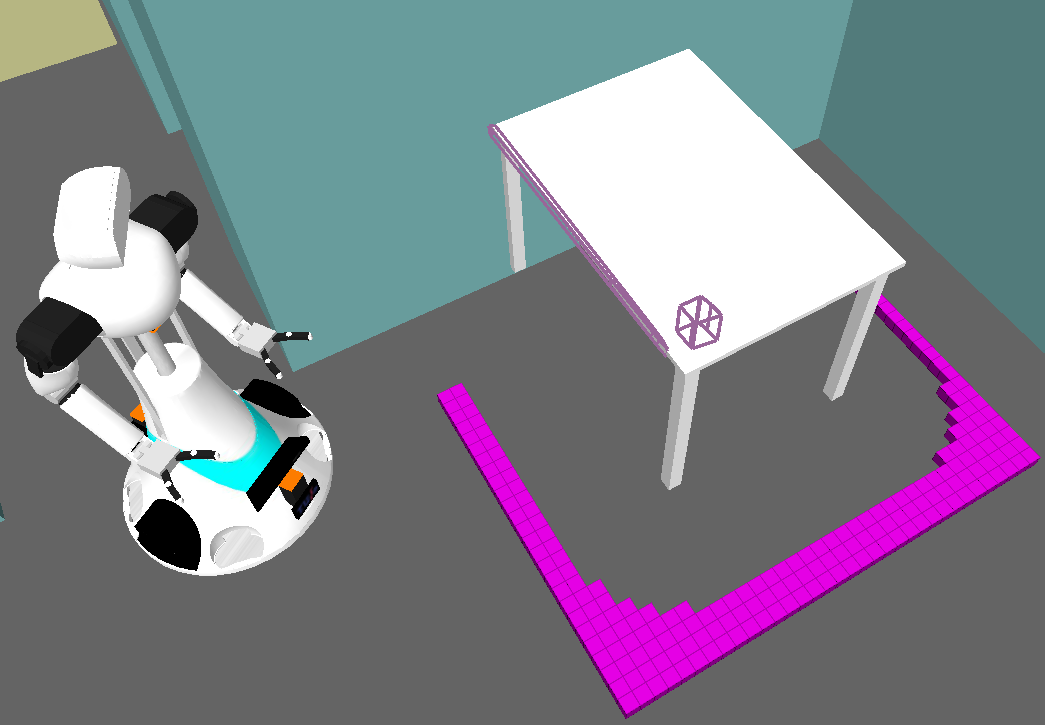
\includegraphics[width=\linewidth]{Figures/constraint_table}
%        \figcaption{Exploration}
%    \end{center}
%\end{minipage}
%\hfill
%\begin{minipage}[T]{0.48\textwidth}
%    \begin{center}
%        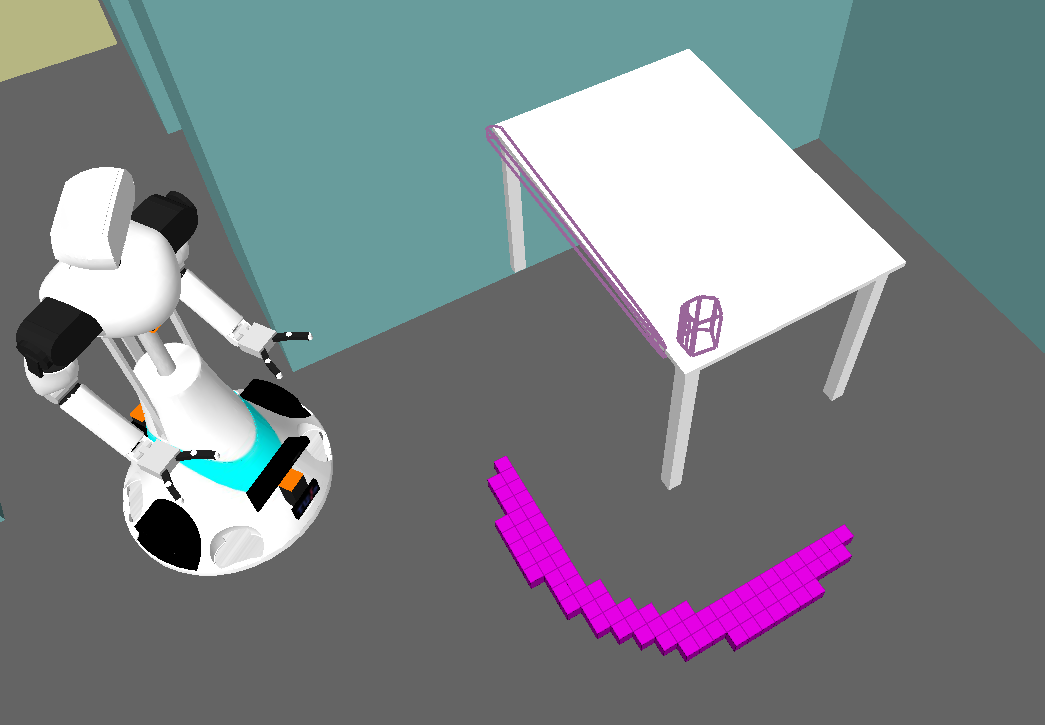
\includegraphics[width=1\linewidth]{Figures/constraint_grasp}
%        \figcaption{Manipulation}
%    \end{center}
%\end{minipage}
\begin{itemize}[itemsep = 0pt, parsep = 0pt, leftmargin=15pt]
	\item Natural Language Interpretation using Feature Context Free Grammar
	\item Speech recognition grammars are deduced from the NLI grammars
%	\item Navigation map: top-down projection of world model entities
%    \item Goals are defined as regions
%    \begin{itemize}[itemsep = 0pt, parsep = 0pt, leftmargin=15pt]
%    	\item Goal region shape depends on task and shape of the world model entity
%    \end{itemize}
%    \item Local planner: DWA with state behavior
%    \begin{itemize}[itemsep = 0pt, parsep = 0pt, leftmargin=15pt]
%    	\item Different behaviors when aligning with the trajectory or arriving at the goal
%    \end{itemize}
\end{itemize}

\end{bclogo}
%
\end{multicols}
\end{slidetop}


\end{document}

